\usecasebase{Pagamento del conto}
\label{usecase:Pagamento del conto}

\begin{figure}[h]
	\centering
	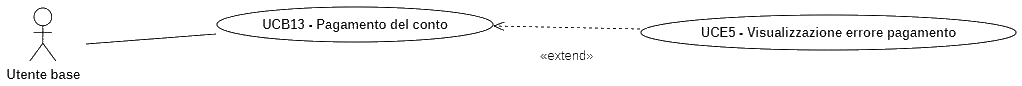
\includegraphics[width=0.9\textwidth]{./uml/UCB13.png} 
	\caption{Pagamento del conto}
	\label{fig:UCB15}
  \end{figure}

\begin{itemize}
	\item \textbf{Attore principale:} Utente base.

	\item \textbf{Precondizione:} L'Utente base ha creato una prenotazione (vedi \autoref{usecase:Prenotazione di un tavolo}), ha 
	scelto come dividere il conto (vedi \autoref{usecase:Selezione della modalità di divisione del conto}) ed inoltre la prenotaziose si deve trovare nello stato "Pagamento".

	\item \textbf{Postcondizione:} L'Utente base ha pagato la sua quota.

	\item \textbf{Scenario principale:}
            \begin{enumerate}
				\item Il Sistema mostra la modalità di divisione del conto scelta per questa prenotazione;
                \item In base alla alla modalità di divisione del conto scelta il Sistema mostra la quota che l'Utente base deve pagare;
				\item L'utente base paga la sua quota premendo il bottone "Paga".
				\item il Sistema mostra un messaggio di conferma del pagamento.
	      \end{enumerate}

    \item \textbf{Scenario secondario:}
		  \begin{itemize}
			  \item \autoref{usecase:Visualizzazione errore pagamento} Errore pagamento:
				\begin{enumerate}
					\item L'Utente base paga la sua quota;
					\item  Il Sistema mostra un messaggio di errore.
				\end{enumerate}
		  \end{itemize}
\end{itemize}